\chapter{Estado del arte}
\label{chap:EstadoArte}

\section{Definición de un negocio minorista}

La distribución comercial minorista es uno de los sectores de mayor relevancia y dinamismo de nuestra economía. Por tanto, es esencial conocer lo que son, a qué se dedican y cómo se gestionan. \\


Un negocio minorista es una empresa que vende productos o servicios directamente a consumidores finales. Los minoristas actúan como intermediarios entre los fabricantes o mayoristas y el mercado de consumo. Sin los negocios minoristas, los productos fabricados a grande escala nunca llegarían a ser consumidos por los clientes finales. El comerciante ofrece un asesoramiento especializado sobre los productos y servicio de su tienda, así como un trato personalizado. \cite{gestionModerna} \\


Además, el comerciante tiene la responsabilidad de conocer cuál es la cantidad de producto que debe comprar para asegurarse de vender lo máximo posible y conseguir con ello un beneficio económico. En algunas ocasiones, también se encarga de establecer los precios de los productos de su tienda. Para ello, se debe tener en cuenta el precio base del producto y se le añade un porcentaje para cubrir los gastos y conseguir beneficios. La otra posibilidad es que los precios de venta al mercado de consumo estén fijados en el etiquetado por los fabricantes. En ese caso, el comerciante no deberá modificar el precio previamente estimado. \\


Podemos clasificar los negocios minoristas según varios criterios, lo cual nos ayudará a entender los tipos que hay y qué funciones tienen cada uno. \\

\textbf{Clasificación de un negocio minorista según su forma de venta \cite{gestionNegocio}: }

\begin{itemize}
	
	\item \underline{Comercio tradicional}:  La mercancía no está a disposición del comprador. El dependiente deberá de proporcionar los artículos al cliente. Podemos identificar tres elementos en este tipo de comercio: el almacén (donde se almacenan los productos), el mostrador (donde se atiende a los clientes) y el vendedor (la persona encargada de asesorar al cliente en sus decisiones de compra y proporcionar el producto al comprador). Ejemplo: carnicerías, farmacias, mercerías, etc. 
	\item \underline{Comercio de libre servicio}: El consumidor tiene libertad para moverse por el espacio de la tienda y elegir los productos a su gusto. En este tipo de comercio el cliente tiene contacto directo con la mercancía, sin intervención del vendedor.  Ejemplos: supermercados, autoservicios, etc. 
	\item \underline{Comercio mixto}: Combina los dos tipos anteriores. El cliente tiene a su disposición la mercancía de la tienda y además el vendedor asesora al comprador sobre sus decisiones dentro de la tienda. Ejemplos: librerías, grandes almacenes, etc. 
	\item \underline{Venta sin establecimiento comercial}: 
	\begin{itemize}
		\item Venta automática: El comprador selecciona un artículo, lo paga y lo recibe en el momento. Ejemplo: Máquina expendedora. 
		\item Venta ambulante: Se realiza en rastros o mercadillos.
		\item Venta a distancia: El comprador adquiere el producto o servicio a través de un medio de comunicación. Ejemplo: Venta por teléfono, venta por Internet, etc. 
	\end{itemize}
\end{itemize}

\textbf{Clasificación de un negocio minorista según su agregación \cite{wikiMinorista}:}

\begin{itemize}
\item \underline{Comercio independiente o pequeño comercio}: Se trata de la tradicional tienda de barrio caracterizada por sus pequeñas dimensiones y por su sistema de venta a través de un mostrador. Funciona de forma autónoma, independiente de otros comercios de su gremio o zona. 
\item \underline{Comercio asociado o comercio integrado}: Son tiendas que se localizan en el mismo local, como los pequeños establecimientos de alimentación que se agrupan en mercados. Los centros comerciales surgen del desarrollo de estas pequeñas asociaciones. 
\item \underline{Gran distribución}: Grandes empresas que actúan al mismo tiempo como mayoristas y minoristas. Generalmente, son grandes multinacionales. EN este tipo se encuentran los hipermercados, con las marcas blancas.
\item \underline{Franquicia}: Tiendas que forman parte de una cadena. Tienen el mismo nombre e imagen y venden productos similares en diferentes ubicaciones. 
\end{itemize}


Con esta clasificación, hemos podido ver que los negocios minoristas recogen un amplio rango de negocios de distinta escala y distinta gestión interna. En concreto, nos centraremos en el estudio de los pequeños comercios mixtos. Entraremos en más detalle en el próximo punto. 

\newpage

\section{Estudio de los pequeños negocios mixtos}

Estos pequeños negocios se caracterizan por el asesoramiento acerca de los productos o servicios que disponen. Uno de los motivos por lo que los consumidores escogen este tipo de tiendas es este, porque les permite tomar una mejor decisión en sus compras. Además, suelen ser negocios menos masificados donde la relación con el cliente toma importancia. \cite{gestionNegocio} \\

Con respecto a la variedad de productos que ofrece un pequeño negocio, es esencial que se especialice y se eliminen los artículos que no sean rentables, así como que se adapte a las características y demandas de sus clientes. Hoy en día, existe una gran competencia con las grandes superficies y la compra online. El comerciante debe ser consciente de esa amenaza y debe ser capaz de distinguirse de las grandes empresas ofreciendo a los clientes unos servicios que no puedan encontrar en otros establecimientos. \\

Los pequeños negocios desarrollan sus propias técnicas de promoción para incentivar y fidelizar clientes. Es su forma de combatir la fuerte competencia entre los negocios y marcas. Estas técnicas se suelen basar en entregar regalos con compras, más cantidad de productos o reducir los precios de estos mediante descuentos. Son acciones que provocan interés en los clientes o consumidores y que les motiva a comprar los productos. 
Para mantener la fidelidad de los clientes, algunos negocios crean formas de promoción basadas en tarjetas de fidelidad, cupones, concursos, etc. Son técnicas tradicionales y comúnmente utilizadas pero dan los resultados esperados. \cite{gago2023dinamizacion} \\

Las formas de pago también pueden ser algo distintas en este tipo de negocios. Como la relación que se establece con el cliente es fuerte, algunas tiendas fían sus productos a los clientes para que puedan probarlos tranquilamente en sus casas, creando confianza y esperando que sean lo suficientemente honestos para devolverlos o pagarlos tras la prueba. \\

La publicidad de estas tiendas suele producirse de forma natural cuando un cliente queda satisfecho y la recomienda a su circulo cercano. Por tanto, una vez más, es crucial el trato que el cliente recibe en este tipo de negocios. Además, se pueden incentivar a nuevos clientes a comprar mediante una página web o las redes sociales. Estas son las técnicas más utilizadas en este tipo de negocios. No necesitan grandes campañas publicitarias puesto que el alcance de un pequeño negocio se limita a los ciudadanos de la localidad donde esté situada la tienda.  \\

Los pequeños negocios tienden a situarse en pequeñas localidades donde la actividad comercial tradicional es favorecida. Los ciudadanos de estas localidades tienen menos facilidades para ir a centros comerciales o grandes franquicias, ya que estas se sitúan en las ciudades. Los pequeños negocios ofrecen los servicios que la población necesita para una vida plena, en la comodidad de su localidad. La facilidad e inmediatez de adquisición de los productos visitando estos pequeños negocios es lo que hace que estas tiendas funcionen bien en este tipo de localidades. \cite{duenas2014calidad} \\


Este proyecto en concreto va destinado al negocio minorista de mi padre. Es una tienda de una pequeña pedanía de Lorca en la que ofrece ropa y calzado para todas las edades, complementos, material de costura y textiles para el hogar. Es una tienda sin empleados, donde el único responsable del funcionamiento de la tienda es mi padre.  

\newpage

\section{Estudio de comerciantes minoristas}

Un estudio realizado por Harvard Business Review demuestra que los emprendedores de 45 años tienen un 85\% más de probabilidades de éxito. Dice que el factor clave de este éxito se debe a la experiencia laboral de los emprendedores de edad media. \\

Para ser capaz de gestionar y administrar un negocio propio es necesario tener unas habilidades y conocimientos que no solo se adquieren recopilando información de los libros, es necesaria tener cierta experiencia en el sector. \cite{autonomos2024master} \\

De este estudio podemos saber que la edad media de los comerciantes minoristas exitosos será superior a los 40 años. En la actualidad, la brecha digital preocupa al 54\% de los mayores de 50 años y la cifra asciende hasta el 76\% en el caso de las personas de más de 80 años, según datos del Observatorio Sénior de 65YMÁS. Por tanto, podemos concluir que algunos comerciantes minoristas sufrirán la becha digital y tendrán dificultades para aprender a usar las nuevas tecnologías. \cite{bbva2024brechadigital} \\

La brecha digital es la desigualdad en el acceso a Internet y las TIC. Hay tres tipos de brecha digital: brecha de acceso (hace referencia a las posibilidades que tienen las personas de acceder a este recurso), brecha de uso (hace referencia a la falta de competencias digitales que impide el manejo de la tecnología) y brecha de calidad de uso (cuando se poseen las competencias digitales para manejarse en Internet, pero no los conocimientos para hacer un buen uso de la red y sacarle el mayor partido posible). La brecha digital se puede dar por la situación geográfica, la diferencia de género, la edad y el nivel económico, entre otros. \cite{iberdrolaBrechaDigital} \\

Como se ha comentado anteriormente, los negocios pequeños suelen darse en pequeñas localidades, donde existe un ambiente más rural y, por tanto, un menor acceso a las TIC. Esto sumado a la edad media de los comerciantes minoristas, nos permite saber que va a existir una evidente brecha digital que habrá de tener en cuenta a la hora de desarrollar una aplicación. 

\newpage

\section{Estudio de usabilidad y accesibilidad}

\subsection{Estudio de usabilidad}

La usabilidad se define formalmente como la medida en que un producto puede ser utilizado por usuarios específicos para lograr objetivos específicos con efectividad, eficiencia y satisfacción en un contexto de uso específico. \cite{iso} \\ 

Cuando hablamos de qué tan buena es una herramienta o sistema, pensamos en los siguientes aspectos \cite{fernandez2018usabilidad}:

\begin{itemize}
	\item \textbf{Efectividad: } Se refiere a la precisión y completitud con las que los usuarios logran ciertos objetivos.
	\item \textbf{Eficiencia: } Esta dimensión mide los recursos expendidos en relación con la precisión y completitud con las que los usuarios logran esos objetivos. Los recursos pueden incluir el tiempo y el esfuerzo físico o mental.
	\item \textbf{Satisfacción: } Engloba la comodidad y aceptabilidad del trabajo para el usuario, considerando también cómo el diseño afecta a la experiencia del usuario en términos de satisfacción.	
\end{itemize}

Mejorar la usabilidad implica entender las necesidades de los usuarios, sus comportamientos y preferencias, y diseñar los productos de manera que faciliten la interacción entre el usuario y el producto.

\subsection{Estudio de accesibilidad}

La accesibilidad en el contexto de diseño web, tecnologías de la información y comunicación se refiere a la capacidad de los sistemas para ser usados por personas con la más amplia gama de capacidades posible. Formalmente, se define como la usabilidad de un producto, servicio, entorno o instalación por personas con la más amplia gama de capacidades". \cite{accesibilidad} \\

Esta definición abarca varios aspectos clave \cite{principios_accesibilidad}: 

\begin{itemize}
	\item \textbf{Diseño universal: } La accesibilidad se logra a menudo a través del diseño universal, que es la práctica de crear productos que sean utilizables por todas las personas, en la mayor medida posible, sin necesidad de adaptación o diseño especializado.
	\item \textbf{Cumplimiento de estándares: } Existen estándares y directrices, como las Pautas de Accesibilidad para el Contenido Web (WCAG), que proporcionan criterios específicos para crear contenido web accesible para personas con discapacidades.
	\item \textbf{Inclusión de capacidades diversas: } La accesibilidad tiene en cuenta una amplia gama de discapacidades.
	\item \textbf{Adaptabilidad: } Capacidad de adaptar y personalizar la interfaz de usuario y el contenido para satisfacer las necesidades individuales de los usuarios.
	\item \textbf{Compatibilidad con Ayudas Técnicas: } Los productos o servicios accesibles deben ser compatibles con las ayudas técnicas utilizadas por las personas con discapacidades, como lectores de pantalla, sistemas de amplificación de sonido, teclados especializados, entre otros.
\end{itemize}

La accesibilidad se fundamenta en el principio de proporcionar un acceso igualitario a la información y a las funcionalidades de un sistema o servicio. Este compromiso no solo facilita la interacción de las personas con discapacidades, sino que también realza la experiencia general de todos los usuarios. En otras palabras, adoptar medidas de accesibilidad no se limita a cumplir con un estándar ético de inclusión; es una práctica que mejora la interfaz y la usabilidad de manera integral, lo que resulta en un diseño más efectivo y universal. \cite{fernandez2021accesibilidad}

\newpage

\section{Legislación actual de protección de datos}

La ley de protección de datos existe para proteger y controlar los datos personales de los usuarios, un derecho fundamental que tienen todas las personas. Esta ley evita que nuestros datos personales sean usados para vulnerar nuestra intimidad u otros derechos fundamentales o libertades. En España esta ley lleva vigente desde el año 2000. \cite{proteccionDatos}\\

Dentro de los datos personales hay distintos niveles de seguridad: bajo, medio y alto. Cada uno de estos niveles tiene distintas medidas de seguridad. Las principales medidas de la ley de protección de datos en España son: 
\begin{itemize}
	\item Solo se deben recoger aquellos datos necesarios para el funcionamiento de la aplicación.  
	\item Se debe avisar a la persona cuáles son los datos que van a ser recogidos y con qué fin van a usarse. 
	\item La persona tiene derecho a dar y deshacer el consentimiento de esos datos si existe una causa justificada. 
	\item Los datos de medio y alto nivel no deben ser recogidos a menos que sea estrictamente necesario. Información como la religión o ideología son datos que no deberían de pedirse. 
	\item La persona que interactúe con datos personales protegidos bajo esta ley deberá de cumplir el secreto profesional. 
	\item Se deben tomar medidas técnicas y organizativas para garantizar la seguridad de los datos en todo momento. 
\end{itemize} 

En nuestro caso concreto, los datos que vamos a pedir a los clientes son únicamente tres campos: el nombre, los apellidos y un número de teléfono, este último de carácter opcional. Son los datos estrictamente necesarios para identificar un cliente. No se pedirán datos innecesarios, como bien postula la ley de protección de datos. 

Puesto que los clientes pueden tomar prestados artículos de la tienda, será necesario un número de teléfono para llamar en caso de que se olviden de devolver o comprar dichos artículos. Si el cliente no quiere dar el número de teléfono o no dispone de uno de ellos, bastará con el nombre y los apellidos. 

Estos datos se almacenarán en una base de datos protegida de manera que se pueda garantizar la seguridad de dichos datos. 


\newpage


\section{Aplicaciones similares y comparativas}


Una de las principales razones para desarrollar esta aplicación es la inexistencia de aplicaciones dedicadas a solucionar los problemas de los pequeños negocios minoristas. Sin embargo, analizaremos a continuación las características de dos de las aplicaciones de gestión de negocios minoristas que hay actualmente en el mercado, para así observar la necesidad de desarrollar una nueva aplicación con unos requisitos distintos. \\

La aplicación más similar que he podido encontrar es myGESTIÓN \cite{myGestion}, el resto de aplicaciones incorporan un punto de venta online que permite a los clientes comprar desde sus casas \cite{clover}. Este punto de venta no sería útil en localizaciones donde el conocimiento tecnológico medio de la población es bajo. Por tanto, se trata de una funcionalidad que complica la aplicación y hace que sea más difícil de usar. Buscamos conseguir una aplicación sencilla que cumpla las necesidades básicas de gestión, siendo así más usable y accesible. Por lo que, aquellas funciones extra que implementan las aplicaciones del mercado actual para negocios más grandes, serán un inconveniente a la hora de establecer un entorno de uso sencillo. Además, un punto importante que no incorporan las aplicaciones de gestión actuales es el sistema de préstamos. Este es un sistema comúnmente utilizado en pequeñas localidades que sí se tendrá en cuenta en el desarrollo de nuestra aplicación. 

\subsection{myGESTIÓN}

myGESTION ofrece una variedad de funcionalidades, incluyendo la gestión de clientes, de artículos y de pedidos de clientes, así como la gestión de ventas, albaranes, facturas y empleados. También incluye un cuadro de mando. Sin embargo, presenta algunos problemas, como la falta de un sistema de préstamos, el exceso de funcionalidades no aplicables a este tipo de negocios y que es un aplicación de pago. 

A continuación se muestra una ilustración que permite ver cómo es la interfaz gráfica de myGESTIÓN. 


\begin{figure}[H]
	\centering
	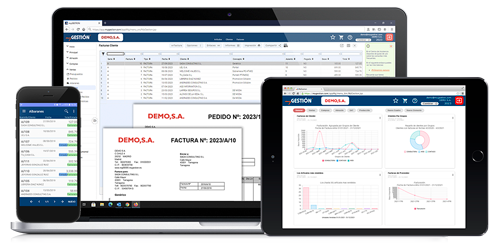
\includegraphics[width=0.8\textwidth]{imagenes/aplicacionesSimilares/caracteristicas-mygestion.png}
	\caption{Interfaz gráfica de myGestión}
\end{figure}

\subsection{Clover}

Clover se centra en la gestión de empleados, clientes y puntos de venta online, además de proporcionar supervisión de inventario. Al igual que myGESTION, Clover enfrenta problemas relacionados con la falta de un sistema de préstamos y tiene funcionalidades que no son necesarias. Además, también es una aplicación de pago.

A continuación se muestra una ilustración que permite ver cómo es la interfaz gráfica de Clover. 

\begin{figure}[H]
	\centering
	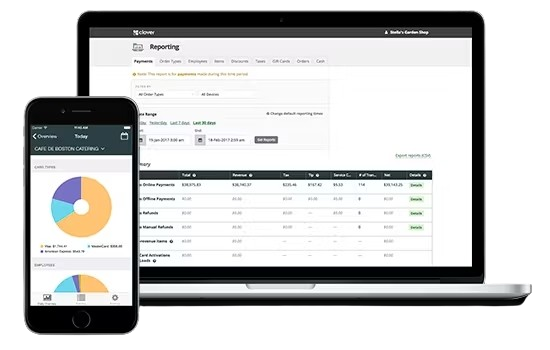
\includegraphics[width=0.8\textwidth]{imagenes/aplicacionesSimilares/clover.png}
	\caption{Interfaz gráfica de Clover}
\end{figure}


\begin{sidewaystable}
	\centering % Centra la tabla en la página
	\begin{tabularx}{\linewidth}{|X|X|X|X|}
		\hline
		\rowcolor{grayshade} 
		\textbf{Nombre de la app} & 
		\textbf{Características principales} & 
		\textbf{Problemas} & 
		\textbf{Plataformas disponibles} \\
		\hline
		myGESTIÓN & 
		\begin{minipage}[t]{\linewidth}
			\begin{itemize}
				\item Gestión de clientes.
				\item Gestión de artículos.
				\item Gestión de pedidos de clientes.
				\item Gestión de ventas, albaranes, facturas.
				\item Gestión de empleados y fichaje.
				\item Cuadro de mando. \\
			\end{itemize}
		\end{minipage} & 
		\begin{minipage}[t]{\linewidth}
			\begin{itemize}
				\item No tiene en cuenta el sistema de préstamos. 
				\item Excedente de funcionalidades, no son necesarios pedidos de clientes ni empleados.  
				\item De pago.
			\end{itemize}
		\end{minipage}  & 
		\begin{minipage}[t]{\linewidth}
			\begin{itemize}
				\item Android
			\end{itemize}
		\end{minipage} \\
		\hline
		Clover & 
		\begin{minipage}[t]{\linewidth}
			\begin{itemize}
				\item Supervisión de inventario.
				\item Gestión de empleados.
				\item Punto de venta online. 
				\item Gestión de clientes. \\
			\end{itemize}
		\end{minipage}  & 
		\begin{minipage}[t]{\linewidth}
			\begin{itemize}
				\item No tiene en cuenta el sistema de préstamos. 
				\item No necesita gestionar empleados. 
				\item No es necesario un punto de venta online, los clientes no lo usarían. 
				\item De pago.\\
			\end{itemize}
		\end{minipage}  & 
		\begin{minipage}[t]{\linewidth}
			\begin{itemize}
				\item Android
				\item iOS
			\end{itemize}
		\end{minipage} \\
		\hline
	\end{tabularx}
	\caption{Descripción de la tabla}
\end{sidewaystable}

